
%%%%%%%%%%%%%%%%%%%%%%%%%%%%%%%%%%%%%%%%%%%%%%%%%%%%%%

\begin{savequote}
The study of Expression is difficult, owing to the movements being often extremely slight, and of a fleeting nature.
\qauthor{Charles Darwin \cite{Darwin2002}}
\end{savequote}

\chapter[Introduction]{Introduction}
\label{ChapterIntroduction}

%%%%%%%%%%%%%%%%%%%%%%%%%%%%%%%%%%%%%%%%%%%%%%%%%%%%%%

\thesiscomment{Thesis Statement (one or two sentences) What is your thesis about and what have you done? If you have a hypothesis what is it? How will you test (prove/disprove) your hypothesis?}

\thesiscomment{Motivation, Why is this problem you've worked on important}

\thesiscomment{Goals / Objectives, What are you trying to do and why? How will you or the reader know if or when you've met your objectives?}

\thesiscomment{Contributions, What is new, different, better, significant? Why is the world a better place because of what you've done? What have you contributed to the field of research? What is now known/possible/better because of your thesis?}

\thesiscomment{The following introduces the recurring themes of the thesis}

\acf{NVC} comprises all forms of intentional, inter-personal communication apart from word based messages and is essential to understand communicated meaning in social situations \cite{Knapp2009} (see Figures \ref{FigureManualGestureNvc} and \ref{FigureGazeNvc} for illustrative examples)\footnote{This definition, together with the alternative perspective of \ac{NVC}  that is independent of intentionality is further discussed in Section \ref{ChapterLiteratureReview}. However, this is a good working definition.}. To enable new ways of intuitively interacting with computers, it would be beneficial for these devices to understand human communication, including \ac{NVC} e.g. using innate communication skills to interact with computer characters. However, this is challenging because human behaviour expression and perception depends on many factors. This thesis describes a study based on the recording and culturally specific\footnote{``culturally specific'' refers to the annotation data being collected from distinct cultural groups of annotators. In this study, the expressors of \ac{NVC} were not divided into distinct cultural groups.} annotation of videos of informal spontaneous conversations, and develops techniques to successfully recognise meaningful communication based on visual non-verbal signals. The use of culturally specific, \continuous labels based on dimensional annotations allows techniques to more faithfully model the culturally specific \ac{NVC} perception of the human observers. ``Continuous value'', in this case meaning ``having an infinite number of possible values'' rather than in the sense of ``continuous recognition'' meaning ``providing a series of predictions based on a temporal series of observations''. \footnote{This is discussed further in Section \ref{SectionDescribeQuestions}.} This results in an approach that can recognise \ac{NVC} signals which is a step towards a system that can be used via common and intuitive communication skills. The four \ac{NVC} signals selected for study were \textit{agree}, \textit{understand}, \textit{thinking} and \textit{question}. This thesis addresses two questions: \textit{how can facial \ac{NVC} signals be automatically recognised}\textit{, given cultural differences in \ac{NVC} perception?} and, \textit{what do automatic recognition methods tell us }\textit{about facial behaviour during informal conversations?}

\begin{figure}[tb]
\centering
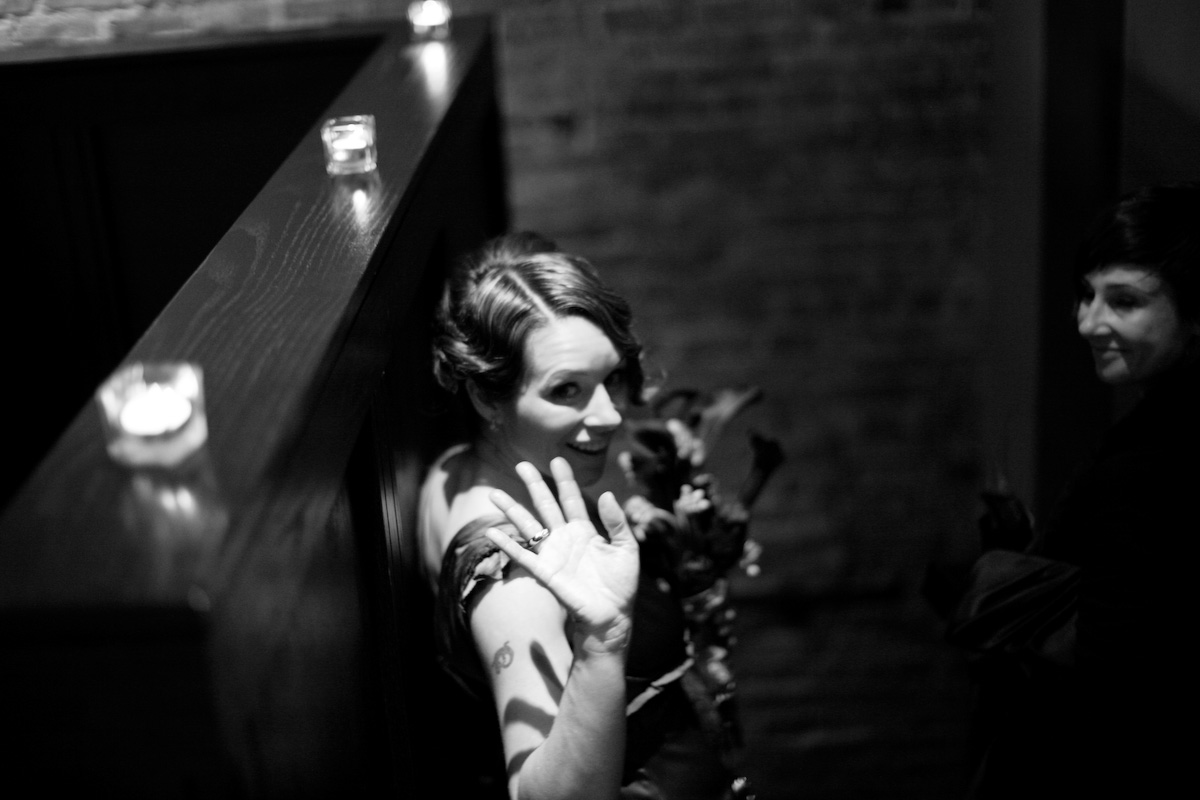
\includegraphics[width = 0.49 \columnwidth]{introduction/wavegoodbye3420075962_ebae9c3a90_o.jpg}
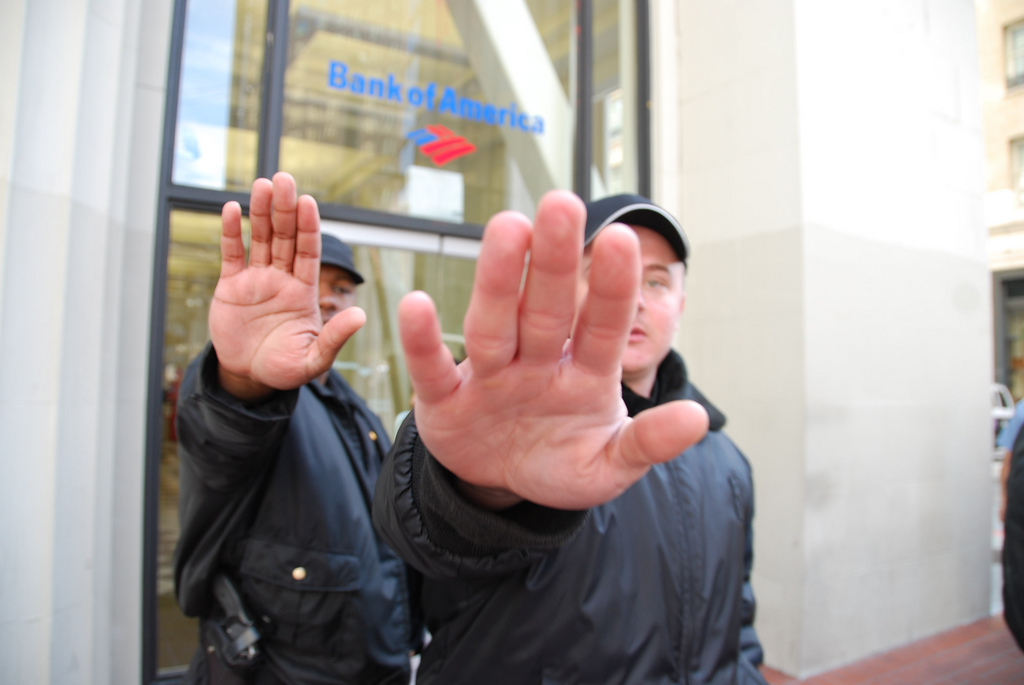
\includegraphics[width = 0.49 \columnwidth]{introduction/security2347593532_a4f7fe8250_b.jpg}
\caption[Hand gestures and facial expressions are often used to convey \ac{NVC}.]{Hand gestures and facial expressions are often used to convey \ac{NVC}. The left photograph shows a woman waving goodbye and smiling. The right photograph depicts two armed security guards with their hands held in a blocking fashion while maintaining eye contact. Photographs used by permission (see Appendix \ref{AppendixPhotoPermissions}).}
\label{FigureManualGestureNvc}
\end{figure}

\section[Motivation: Why Attempt Automatic Recognition?]{Motivation: Why Attempt Automatic Recognition of \ac{NVC}?}

Computers are becoming pervasively used in society because of their portability, connectivity and low cost. They are being integrated into many common home appliances, including cars, mobile phones and televisions. \ac{NVC} is a communication skill that almost all humans possess and may be used to operate computers if the appropriate interfaces are available. Furthermore, if human to human communication can be understood by a device, it may be possible for it to support or analyse the interaction \cite{Nakatsu98}. Existing \ac{HCI} interfaces do not necessarily extend to multiple embedded computers, and particularly to those without traditional physical input controls \cite{Pantic2008}. Potential applications of automatic \ac{NVC} recognition and emotionally aware computing include:

\begin{itemize}
 \item Computer generated characters and robots capable of a fully interactive conversation, including perception and expression of \ac{NVC} and emotion \cite{Pantic2009}. Early prototypes of this concept include the {SEMAINE} Sensitive Artificial Listener \cite{Schroder2011} and Asimo the robotic museum guide \cite{Asimo2013}. The computer character could be used for entertainment, companionship or for providing information and assistance.
 \item Monitoring of social human behaviour and automatically providing services which are useful and appropriate for the social context. This could be in the form of advice, information or assistance \cite{Liao2006}. Computer may be able to optimise work patterns and reduce untimely interruptions \cite{Horvitz2003}. Emotionally aware computers may also provide an opportunity to practice social skills \cite{Hopkins2011}.
 \item Computer based learning can detect if a human is confused or bored and adapt the teaching style accordingly \cite{DMello2007}.
 \item Human operator monitoring in safety critical situations can detect tiredness, confusion or ignoring important information. This can be applied to transportation (cars \cite{Ji2004}, aircraft, etc.), industrial machinery or any safety critical device.
 \item Text entry based on audio-visual speech recognition. Because of the association between words, emotions and \ac{NVC} \cite{Cowie1999, Jones99}, a hybrid recognition approach could improve speech recognition performance.
 \item Automatic labelling of broadcast material, based on the behaviour of the people featured in the footage, or from the reaction of observers \cite{Pantic2009b}.
\end{itemize}

Applications of automatic \ac{NVC} and behaviour recognition systems, in which the result is directly interpreted by humans include:

\begin{itemize}
 \item Product evaluation. As a person interacts with a product, their reactions, emotions, mental state and intentions can be automatically recognised which provides useful information for evaluating a product's appeal \cite{Mano1993}.
 \item Security applications. Behaviour monitoring \cite{Pfister2011}, covert lip reading \cite{Ong2011} and lie detection can be used by police for crime detection. The work contained in this thesis originated from the EPSRC LILiR project, which developed video based lip reading technology.
 \item Human behaviour research. Higher level patterns in behaviour can be quickly analysed if low level \ac{NVC} behaviour can be automatically recognised \cite{Okwechime2011}.
\end{itemize}

Automatic \ac{NVC} recognition has a wide range of potential applications but these are often in roles that are quite different from existing computer systems. If human behaviour is to be automatically recognised, the issue of context and situational dependence of human behaviour must be considered.

\section{From the Laboratory to the World (or Why Automatic \ac{NVC} Recognition is Difficult)}
\label{BackgroundWhyIsNvcDifficult}
\label{BackgroundNaturalConvesationContainsRapidHeadMotion}

\begin{figure}[tb]
\centering
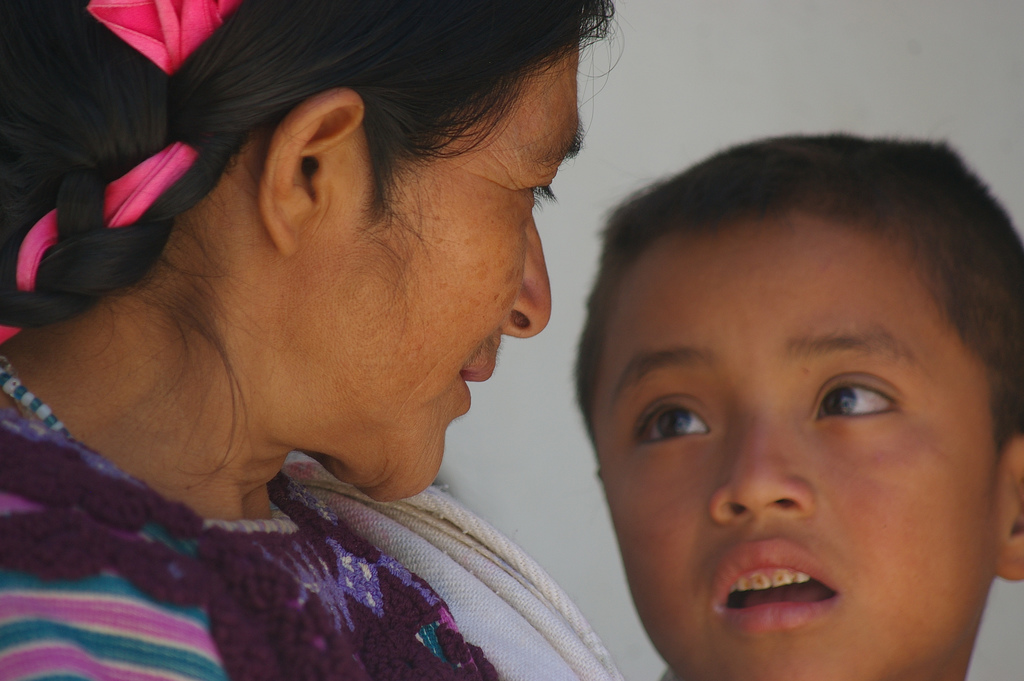
\includegraphics[width = 0.59 \columnwidth]{introduction/eyecontact2503079623_0a4aecf3c9_b.jpg}
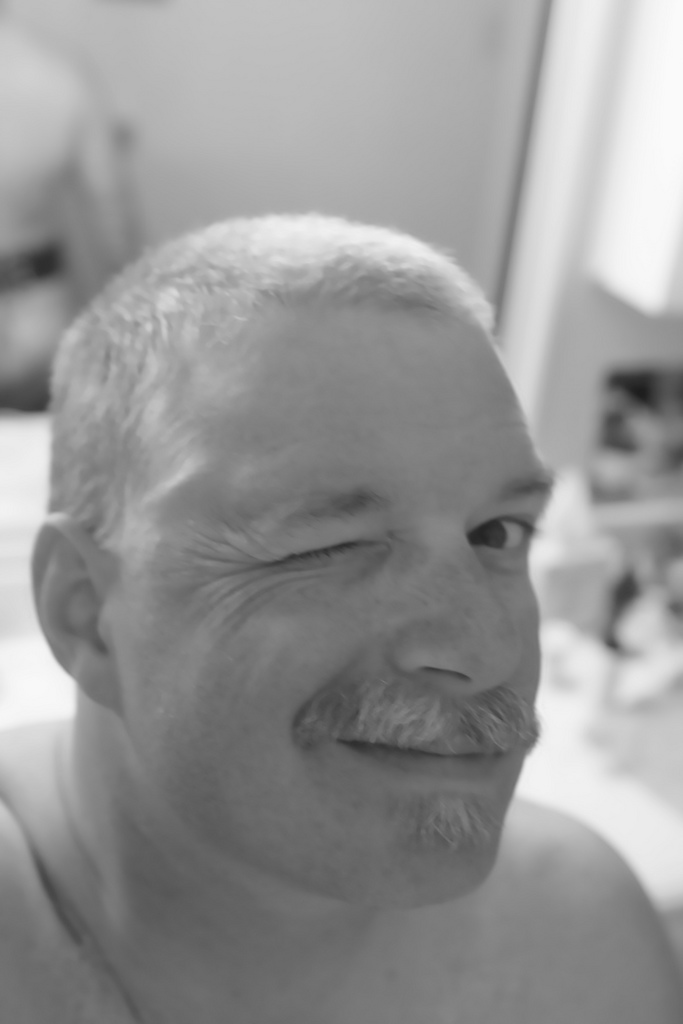
\includegraphics[width = 0.29 \columnwidth]{introduction/wink3083102723_2180fe13c6_b.jpg}
\caption[Eye contact has a significant role in \ac{NVC}.]{Eye contact has a significant role in \ac{NVC}. The left photograph shows a mother and child during mutual eye contact. The proximity and body pose of the people implies a close intimacy. The right photograph shows a man winking, which is often intended as a sign of trust. Photographs used by permission (see Appendix \ref{AppendixPhotoPermissions}).}
\label{FigureGazeNvc}
\end{figure}

%This section summarises the main challenges in creating an effective \ac{NVC} system. 
The way \ac{NVC} is expressed and perceived depends on the context in which it is used e.g. certain types of behaviours may be considered as inappropriate in specific social situations and not be expressed, as well as behaviour such as nodding, winking, kissing, nodding, etc. that are interpreted depending on the social relationship\footnote{This is discussed more fully in Section \ref{BackgroundWhatFactorsInfluenceNvc}.}. Many studies of automatic human behaviour recognition use posed data recorded in a laboratory environment \cite{Pantic2009, GaticaPerez2009, Vinciarelli2008}. Posed \ac{NVC} data differs significantly from natural data. These differences include the types of communication actions used, expression intensity, the style of expression and in the timings of gestures. To maximise the range of applications in which the automatic system can be applied, this thesis attempts to use spontaneous human behaviour where possible.

%At the time when this work was conducted, there existed no public dataset that was suitable for studying the automatic recognition of \ac{NVC} in a naturalistic and spontaneous social context. This was because all other datasets, apart from a part of the AMI meeting corpus \cite{Carletta2007}, were either were posed expressions, featured multiple social contexts or were recorded in a contrived social context. The most similar dataset was the naturalistic portion of the AMI meeting corpus, although this was not ideal for facial feature tracking, as is discussed later in Chapter \ref{ChapterCorpus}. 

At the time this work was conducted, there were limited available public data sets that would support the research. Data sets have been recorded in many different social situations with different degrees of spontaneity and naturalness. The most viable existing candidate was the AMI meeting corpus \cite{Carletta2007} (discussed in detail in Section \ref{SectionExistingDataSets} along with other relevant data sets). However, only a portion of this corpus is naturalistic and it was not suitable for the tracking method employed in Chapter \ref{ChapterClassification} and subsequent chapters. A new dataset that was suitable for this study was created. This thesis attempts to use a specific social context because behaviour is expression and perception is dependent on social context. A context was chosen that may have useful applications i.e. it is a commonly experienced situation that is important for interpersonal relationships. Also, the selected social situation should be easily reproducible in order to reduce resources requirements and to enable future work in the same social context. However, database recording and annotation is a challenging task due to the sensitivity of humans to context, practical considerations when recording usable video and audio, and the resource requirements for annotation \cite{Cowie2005}. A new corpus was recorded based on informal conversations between two people. This corpus was publicly released to assist further research.

Context is significant in determining the way people perceive \ac{NVC} \cite{Hoque2009}. One significant contextual factor is culture \cite{Matsumoto08}; different cultures often have unique meaningful gestures \cite{Matsumoto2006}. If a single group of annotators is used and the ratings of annotators combined to form a group specific consensus label, these perceptual cultural differences would be ignored. Using annotators from a single culture results in annotations based on perceptions that are specific to that culture. An alternative would be to use independent sets of expressors and annotations, each set from the same culture. This would allow studies to identify \ac{NVC} signals specific to that culture. However, the creation of such a dataset is beyond the scope of this thesis which focuses on cultural perception differences. To account for the cultural differences in perception, observers from three different cultures were used to create \culturallySpecific annotations. This can be used as a basis for training and testing automatic recognition systems that are better suited to recognise \ac{NVC} in a way that is more like a human observer. This is shown by confirming the presence of cultural differences in the annotation data\footnote{see Table \ref{MeanAnnotatorCorrelationTable}} and the automatic system trained on a specific culture is better at recognising \ac{NVC} signals\footnote{see Table \ref{CrossCulturePerformanceTable}}.

Automatic recognition of \ac{NVC} is difficult because there are many possible ways of expressing a particular \ac{NVC}. Each person has a particular style of expression \cite{Buck1979}, as well as being influenced by many contextual factors. During most social situations, there are multiple sources of body and face motion that do not relate to \ac{NVC}, including lip movement caused by speaking, ambient motion (small body movements that are continuously present, e.g. breathing) and the subset of emotions which are not involved in \ac{NVC}. As Krauss \etal \cite{Krauss1996} said ``All hand gestures are hand movements, but not all hand movements are gestures[...]''.  \ac{NVC} signals are expressed with a duration ranging from a fraction of a second to several hours \cite{Aaron1997, Verduyn2009}. \ac{NVC} also involves visual, audio, tactile and other signals to convey messages \cite{Knapp2009}. It can be difficult to encode all this information in a form that is suitable for machine learning. This makes the learning of associations between gestures and \ac{NVC} meaning very challenging. This thesis focuses on visual information in the human face. These visual signals are rich in \ac{NVC} information but considering the face exclusively is far from being a comprehensive view of \ac{NVC}.

\section{Main Thesis Contributions}

To address these challenges, the main contributions of this thesis are:

\begin{enumerate}
 \item The design and publication of a new corpus to study human behaviour in an informal social situation. Minimal constraints on participants were imposed to allow spontaneous, natural conversation, which is necessary to gather data that is suitable to study \ac{NVC}. The corpus is publicly available for further use\footnote{\scriptsize{http://www.ee.surrey.ac.uk/Projects/LILiR/twotalk\_corpus/}} \cite{SheermanChase2009}. This database differs from previously available datasets (discussed in Section \ref{SectionExistingDataSets}).
 \item A crowd-sourced method for multi-cultural annotation. This provides a basis for studying automatic \ac{NVC} recognition from different cultural perceptions. The labels used for annotation were based on \ac{NVC} message meaning. Cultural differences in \ac{NVC} perception were found to be present.
%This process resulted in a annotation consensus in four dimensional, continuously valued set of labels which encode \ac{NVC} meaning.
 \item Design and evaluation of an automatic system for \ac{NVC} meaning recognition. Various feature extraction methods and classifiers were compared to find an effective approach. \ac{NVC} recognition was also approached from a regression perspective to produce \continuous label predictions. Effective performance was observed using a system based on tracking facial features, computing distances between pairs of trackers, then forming features based on their statistical properties as the basis for regression. Feature selection was also employed and found to significantly improve performance. Using an automatic system trained on \culturallySpecific annotation data was found to result in a higher performance than using annotations from a different culture.
 \item Automatic techniques that were developed as part of the recognition system were applied to automatically identify patterns of human behaviour. The presence of interpersonal coordination in human behaviour was confirmed and quantified for the face. The feature components that were most relevant for \ac{NVC} recognition were identified. Analysis was performed using both quantitative methods and by direct visualisation of facial regions involved.
\end{enumerate}

The outcomes of the thesis are:

\begin{enumerate}
 \item a new, publicly available \ac{NVC} corpus that has been annotated by people from different cultures,
 \item provided additional evidence that there are cultural differences in \ac{NVC} perception, 
 \item an effective method for natural \ac{NVC} recognition and
 \item demonstration that culturally specific \ac{NVC} recognition models leads to higher performance.
\end{enumerate}

\section{Overview of Thesis}

Chapter \ref{ChapterLiteratureReview} discusses existing research relating to \ac{NVC}, classification, machine learning and \featureGeneration. The recording of the \ac{NVC} corpus is discussed in Chapter \ref{ChapterCorpus}. This corpus is then used as a basis for studying automatic classification, as described in Chapter \ref{ChapterClassification}. Chapter \ref{ChapterBackchannel} investigates the effect of interpersonal coordination of behaviour between the two conversation participants, and attempts to use the reaction of a person to infer the \ac{NVC} of an unseen subject. Collection of annotation data from culturally distinct groups is described in Chapter \ref{ChapterAnnotation}. This annotation data is used in a study of a culturally specialised regression as discussed in Chapter \ref{ChapterNvcRegression}. The facial deformation is encoded using a geometry based feature extraction method but this feature contains redundant and irrelevant information. Chapter \ref{ChapterFeatureSelection} uses feature selection to isolate a set of features that improves \ac{NVC} regression performance. General conclusions are drawn in Chapter \ref{ChapterConclusion}.

